\documentclass[pdf]{beamer}
\mode<presentation>{
	\usetheme{Ilmenau}
	
}
\usecolortheme{dolphin}
%\usepackage[UTF8,indent]{ctexcap}%中文
\usepackage{amssymb}
\usepackage{amsmath}
\usepackage{amsfonts}
%\usepackage{graphicx}
\usepackage{amsthm}
\usepackage{indentfirst}
\usepackage{enumerate}
\usepackage{extpfeil}
\usepackage{tikz-cd}
\usepackage{longtable}
\usepackage{makecell}
\usepackage{TooYoung}
\usepackage{array}
\usepackage{xcolor}
\usetikzlibrary {calc,positioning,shapes.misc,graphs,decorations.pathreplacing}


\numberwithin{equation}{section}

\theoremstyle{plain}
\newtheorem{proposition}[theorem]{Proposition}
\newtheorem{claim}[theorem]{Claim}
\newtheorem{defn}[theorem]{Definition}
\newtheorem{eg}[theorem]{Example}
\newtheorem{pf}[theorem]{Proof}
\newtheorem{cor}[theorem]{Corollary}

\newtheorem{tabloid}[theorem]{Tabloid: equivalence class of standard filling}


\theoremstyle{plain}
\newtheorem{exercise}{Exercise}[section]


\theoremstyle{remark}
\newtheorem{remark}[theorem]{Remark}
\newtheorem{remarks}{Remarks}
\newtheorem{ex}[theorem]{Exercise}
\newtheorem{question}[theorem]{Questions}
\newtheorem{short}{ }



\newcommand*{\thick}[1]{\text{\boldmath$#1$}}
\newcommand*{\cir}[1]{\;$\ding{19#1}$\;}%临时使用
\newcommand*{\norm}[1]{\lVert#1\rVert}
\newcommand*{\ignore}[1]{\textcolor{lightgray}{#1}}
\newcommand*{\stress}[1]{\textcolor{red}{#1}}
\newcommand*{\bgpicb}[1]{\usebackgroundtemplate{%
	\begin{tikzpicture}[path image/.style={
		path picture={
			\node at (path picture bounding box.center) {
				\includegraphics[height=10cm]{#1}
			};
	}}]
	
	\draw [path image]
	(current page.north west) rectangle
	(current page.south east);
	
	\end{tikzpicture}
}}
\newcommand*{\bgpica}[1]{\usebackgroundtemplate{%
		\begin{tikzpicture}[path image/.style={
			path picture={
				\node at (path picture bounding box.center) {
					\includegraphics[height=7.5cm]{#1}
				};
		}}]
		
		\draw [path image]
		(current page.north west) rectangle
		(current page.south east);
		
		\end{tikzpicture}
}}


\DeclareMathOperator{\supp}{supp}
\DeclareMathOperator{\dist}{dist}
\DeclareMathOperator{\vol}{vol}
\DeclareMathOperator{\diag}{diag}
\DeclareMathOperator{\tr}{tr}
\DeclareMathOperator{\Proj}{\operatorname{Proj}}
\DeclareMathOperator{\Aut}{\operatorname{Aut}}
\DeclareMathOperator{\Img}{\operatorname{Im}}
\DeclareMathOperator{\Sym}{\operatorname{Sym}}
\DeclareMathOperator{\sgn}{\operatorname{sgn}}
\DeclareMathOperator{\Id}{\operatorname{Id}}
\DeclareMathOperator{\ques}{\;?\;}
\DeclareMathOperator{\Fl}{\mathcal{F\ell}}
%\setlength{\parindent}{1em}
\newcommand{\character}[2]{\left[\begin{array}{c}{#1} \\ {#2}\end{array}\right]}
\newcommand{\normalcharacter}{\character{\epsilon}{\epsilon'}}
\renewcommand{\Fontinbox}[1]{\scriptstyle #1}


\setbeamertemplate{caption}[numbered]
% 设置图形文件的搜索路径
\graphicspath{{figures/}}
\title{Springer Fibers for $SL_n(\mathbb{C})$}
\author{Xiaoxiang Zhou}
\institute[Bonn uni]{Universität Bonn}
\date{January 9, 2023}
\tikzset{
	invisible/.style={opacity=0,text opacity=0},
	visible on/.style={alt=#1{}{invisible}},
	alt/.code args={<#1>#2#3}{%
		\alt<#1>{\pgfkeysalso{#2}}{\pgfkeysalso{#3}} % \pgfkeysalso doesn't change the path
	},
}
%\setbeamercolor{section number projected}{fg=white!90!blue, bg=red!90!black}
\definecolor{goodblue}{RGB}{71,71,186}
\setbeamercolor{block body}{fg=black,bg=gray!10}
\setbeamercolor{block title}{fg=white, bg=goodblue}
\usefonttheme[onlymath]{serif}
\usepackage[T1]{fontenc}
\usepackage{lmodern}

\setbeamertemplate{headline}{
	\begin{beamercolorbox}[wd=\paperwidth,ht=2.5ex,dp=1.125ex]{section in head/foot}%
		\hspace{3ex}{\insertsectionhead}
	\end{beamercolorbox}
	%	\begin{beamercolorbox}[ht=2.5ex,dp=1.125ex,leftskip=.3cm,rightskip=.3cm plus1fil]{subsection in head/foot}
	%		\usebeamerfont{subsection in head/foot}\insertsubsectionhead
	%\end{beamercolorbox}
}%删除点
\begin{document}
\begin{frame}
	\titlepage
\end{frame}
\begin{frame}[fragile]{Recap: representation theory of finite groups}
Restrict to \textbf{complex} representations, we have a nice theory:

\begin{itemize}
	\item Any representation can be written as a direct sum of \textbf{irreducible representation};
	\item We can extract information of irreducible representations from the \textbf{character table}:\\[-0.5cm]
	\begin{equation*}
	\begin{aligned}
	\#\{ \text{irreducible representations} \} =& \#\{ \text{conjugation classes} \}\\
	\sum_{\chi: \text{irr}} (\dim \chi)^2 =& \#G
	\end{aligned}
	\end{equation*}
	
\end{itemize}
However, in general, 
\begin{itemize}
	\item NO standard way finding an \textbf{explicit construction} of all irreducible representations; 
	\item NO \textbf{one-to-one correspondence} between irreducible representations and conjugation classes.
\end{itemize}
\end{frame}
\begin{frame}

	In this talk, we use two methods to understand representations of $S_n$, and find connections/analogs between them.

\begin{table}[ht]
	\centering
\begin{tabular}{c|c}
	\Xhline{1.2pt} 
	methods & objects \\
	\Xhline{0.8pt} 
	combinatorial & Young diagram, Young tableau\\
	\hline
	geometrical & Springer fiber of $SL_n(\mathbb{C})$, irreducible components\\
	\Xhline{1.2pt} 
\end{tabular}
\end{table}

\end{frame}
%\begin{frame}{Contents}
%\tableofcontents
%\end{frame}



%\begin{frame}{Goal \ignore{of the Part I}}
%	\begin{itemize}
%		\item Explicitly construct irreducible representations of $S_n$ 
%		
%		by Young diagram;
%		\item Compute the character table;
%		\begin{itemize}
%			\item $\dim \chi_i$ \hspace{1cm}\ignore{by recursion / Hook length formula}
%			\item character \hspace{.65cm}\ignore{by Frobenius formula}
%		\end{itemize}
%	
%	\item Compute other representations.
%	\begin{itemize}
%		\item e.g. $\otimes,\, \Sym^m,\, \Lambda^m$;
%		\item e.g. $M_{\lambda}$.
%		\item \ignore{restriction and induced representation}
%	\end{itemize}
%	\end{itemize}
%\end{frame}
\begin{frame}{Goal \ignore{of the Part I}}
\begin{itemize}
	\item Explicitly \stress{construct irreducible representations} of $S_n$ 
	
	by Young diagram;
	\item Compute the character table;
	\begin{itemize}
		\item $\dim \chi_i$ \hspace{1cm}by recursion \ignore{/ Hook length formula}
		\item \ignore{character \hspace{.65cm}by Frobenius formula}
	\end{itemize}
	\item \ignore{Compute other representations.}
		\begin{itemize}
			\item \ignore{e.g. $\otimes,\, \Sym^m,\, \Lambda^m$;}
			\item \ignore{e.g. $M_{\lambda}$.}
			\item \ignore{restriction and induced representation}
			\item \ignore{representation ring}
	\end{itemize}
\end{itemize}
\end{frame}
%\usebackgroundtemplate{%
%	\begin{tikzpicture}
%	\useasboundingbox (current page.north west) rectangle
%	(current page.south east);
%	\draw[fill, green]  (current page.center) circle [radius = 4cm];
%	\end{tikzpicture}
%
%}

\begin{frame}[fragile]{Notation}
For boxes:
\renewcommand{\Fontinbox}[1]{\scriptstyle #1}
\begin{figure}[h]
	\centering
	\begin{tabular}{ccc}
		(Young) diagram & filling & standard filling  \\
		$\Yng(3,2)$ & $\Young{\scriptstyle11&78&11\\6&8}$ & $\Young{3&5&4\\1&2}$  \\
		& tableau & standard tableau \\
		& $\Young{6&11&11\\8&78}$ & $\Young{1&3&4\\2&5}$
	\end{tabular}
\end{figure}
Order of Young diagram:
\renewcommand{\Fontinbox}[1]{\scriptscriptstyle #1}
\begin{figure}[h]
	\centering
	\setlength\Youngwidth{0.5pc}\setlength\Youngheight{0.5pc}
	\begin{tabular}{ccc}
		inclusion & dominance & Lexicographic ordering  \\[0.2cm]
		$\Young{&&\\&\\[]} \raisebox{1mm}{$\,\subseteq\,$} \Young{\hook[c]&\hook[c]&\hook[c] & \\ \hook[c] & \hook[c] \\}$  & $\Young{&&\\&&[]\\[]\\[]\\[]\\[2]&[4]&[5]} \raisebox{4mm}{$\,\trianglelefteq\,$} \Young{&\\ \\ \\\\[]\\ [4] & [5] & [5]}$ & $\Young{&&\\&&\\[]\\[]\\[2]&[\textcolor{gray}{4}]&[\textcolor{gray}{6}]&[\textcolor{gray}{6}]} \raisebox{3.5mm}{$\hspace{-1.5mm}\leqslant\,$} \Young{&&&\\\\\\[]\\[{3}]&[\textcolor{gray}{4}]&[\textcolor{gray}{5}]&[\textcolor{gray}{6}]}$  \\
	\end{tabular}
\end{figure}

\end{frame}
\begin{frame}{tree of Young diagram}

\end{frame}
\bgpicb{figure/youngdiagram0.pdf}
\begin{frame}{tree of Young diagram\quad\hyperlink{skiporder}{\beamergotobutton{skip}}}

\end{frame}
\bgpicb{figure/youngdiagram_order.pdf}
\begin{frame}{Order}
$\subseteq$ inclusion \\
$\trianglelefteq$ dominance \\
$\leqslant$ Lexicographic ordering\\
\vspace{10cm}
\end{frame}
\usebackgroundtemplate{}
\begin{frame}[label=skiporder]{$S_n$ \& Young diagram}
 \begin{overlayarea}{\linewidth}{\textheight}
\only<1-2>{\begin{proposition}
	We have the one-to-one correspondence
	$$\left\{ \begin{gathered}
	\text{Young diagram}\\\text{of $n$ boxes}
	\end{gathered}  \right\} \underset{\lambda=\lambda_1^{v_1} \cdots \lambda_k^{v_k}}{\xleftrightarrow{\text{partition of $n$}}}\left\{ \begin{gathered}
	\text{Conjugation class}\\\text{of $S_n$}
	\end{gathered}  \right\}$$
\end{proposition}}
\only<1>{\begin{eg}
	$n=11.$
	$$\Yng(5,4,1,1)\underset{\lambda=5\cdot 4\cdot 1^2}{\xleftrightarrow{11=5+4+1+1}} (12345)(6789)(10)(11)\hspace{-9mm}$$
\end{eg}}
\only<2,3>{\begin{claim}
	$$\left\{ \begin{gathered}
	\text{Young diagram}\\\text{of $n$ boxes}
	\end{gathered}  \right\} \xleftrightarrow{\quad?\quad}\left\{ \begin{gathered}
	\text{Irreducible rep}\\\text{of $S_n$}
	\end{gathered}  \right\}$$
\end{claim}}
\only<3>{\begin{remark}
		Reduced to: for each Young diagram $\lambda$, \\
		\phantom{Reduced to:} construct an irreducible representation $S^{\lambda}$, and \\
		\phantom{Reduced to:} prove $S^{\lambda}=S^{\lambda'} \Rightarrow \lambda=\lambda'.$
\end{remark}}
\end{overlayarea}
\end{frame}



\begin{frame}[fragile]{The construction of $S^{\lambda} \subseteq M^{\lambda}$}
 \begin{overlayarea}{\linewidth}{\textheight}
 	\only<1>{
\begin{tabloid}
%	$$\setlength\Youngvline{0pt}\Young{3&5&4\\1&2} = \Young{3&4&5\\2&1} = \Young{3&4&5\\1&2} :=\{345/12\}$$

\includegraphics[width=\linewidth]{figure/shadow/tabloid.png}
\end{tabloid}
\begin{block}{}
	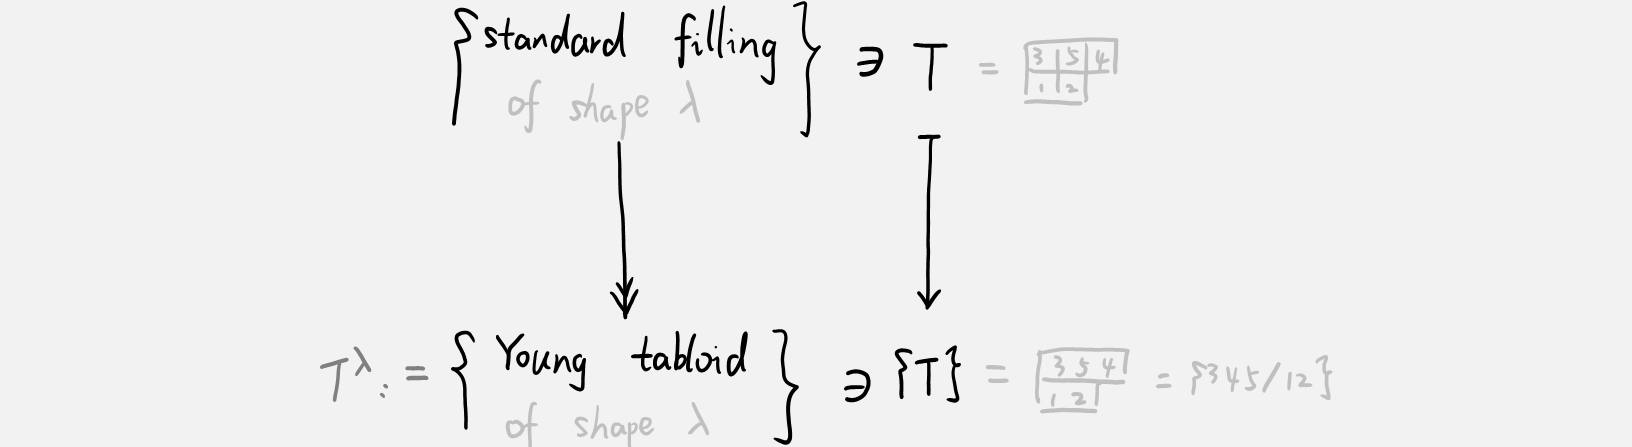
\includegraphics[width=\linewidth]{figure/shadow/tabloid2.png}
\end{block}}


	 	\only<2-4>{\begin{block}{}
	 	\only<2-3>{
	\begin{equation*}
	\begin{aligned}
		\mathcal{T}^{\lambda}:=& \left\{\text{Young tabloid of shape }\lambda \right\}\\
		M^{\lambda}:=& \left< \{T\} \in \mathcal{T}^{\lambda}\right>_{\mathbb{C}} \quad   \\
	\end{aligned}
\end{equation*}}
 	\only<2,4>{
 	\only<2>{Choose a standard filling $T$ of shape $\lambda$,}
	\begin{equation*}
\begin{aligned}
 	\only<4>{&\\[-1cm]}
	 	\only<2>{C(T):=&\left\{\sigma \in S_n\middle|\, \sigma \text{ preserves numbers in each column} \right\}\\}v_{T}:= & \sum_{\sigma \in C(T)}\sgn(\sigma) \{\sigma \cdot T\} \in M^{\lambda}
	\qquad\qquad\qquad \only<4>{\ignore{\sigma v_T = v_{\sigma T} }}
	  \\
	S^{\lambda}:=& \;\mathbb{C}[S_n]\cdot v_T \subseteq M^{\lambda} \qquad\qquad \ignore{\text{invariant subspace of $M^{\lambda}$}}
	\end{aligned}
	\end{equation*}}
\end{block}}
 	\only<3>{
\begin{eg}[$\lambda=3 \cdot 2$]
		$\,$\\[-1cm]
		\begin{equation*}
	\begin{aligned}
	\mathcal{T}^{\lambda}=& \left\{\begin{gathered}
	\{123/45\}, \{124/35\}, \{125/34\}, \{134/25\},\{135/24\}, \\
	\{145/23\}, \{234/15\}, \{235/14\}, \{245/13\},\{345/12\}\phantom{,} \\
	\end{gathered}\right\}\\
	M^{\lambda}=& \left<\begin{gathered}
	\{123/45\}, \{124/35\}, \{125/34\}, \{134/25\},\{135/24\}, \\
	\{145/23\}, \{234/15\}, \{235/14\}, \{245/13\},\{345/12\}\phantom{,} \\
	\end{gathered}\right>_{\mathbb{C}}\\
	\end{aligned}
	\end{equation*}
\end{eg}
}
\renewcommand{\Fontinbox}[1]{\scriptscriptstyle #1}
 	\only<4>{	
	\begin{eg}[$\lambda=3 \cdot 2$]
	\setlength\Youngwidth{0.6pc}\setlength\Youngheight{0.6pc}
		$\,$\\[-0.8cm]
		\begin{equation*}
		\begin{aligned}
		T = & {\Young{3&5&4\\2&1}}\\
		C(T) =&\left\{ \Id, (23), (15), (23)(15)  \right\}\\
		v_T= & \big\{\Young{3&5&4\\2&1} \big\} - \big\{\Young{2&5&4\\3&1} \big\} - \big\{\Young{3&1&4\\2&5} \big\} + \big\{\Young{2&1&4\\3&5} \big\} \\
		=& \{345/12\}-\{245/13\}-\{134/25\}+\{124/35\} \in M^{\lambda}\\
		S^{\lambda}=&\left<  v_T  \right>_{\mathbb{C}[S_n]} = \left<  v_{T'} \middle| T': \text{standard filling}  \right>_{\mathbb{C}}
		\end{aligned}
		\end{equation*}
	\end{eg}
}
\end{overlayarea}
\end{frame}

\begin{frame}{Main theorem of $S^{\lambda}$}
\begin{theorem}
	Fix the Young diagram $\lambda$, the corresponding representation $S^{\lambda}$ has the following properties:
	\begin{enumerate}
		\item the linear space $S^{\lambda}$ has a \textbf{basis} $\left\{  v_{T'} \middle| T': \text{standard tableau} \right\}$,\\
		especially, $\dim S^{\lambda}= \# \{\text{standard tableau}\}$;
		\item the representation $S^{\lambda}$ is \textbf{irreducible};\\
		\item for the Young diagram $\lambda'$, $S^{\lambda'} \cong S^{\lambda} \Rightarrow \lambda'=\lambda$.
	\end{enumerate}
\end{theorem}

\end{frame}
\begin{frame}{Proof: basis}
\begin{theorem}
		\begin{enumerate}
		\item the linear space $S^{\lambda}$ has a basis $\left\{  v_{T'} \middle| T': \text{standard tableau} \right\}$,\\
		especially, $\dim S^{\lambda}= \# \{\text{standard tableau}\}$;
	\end{enumerate}
\end{theorem}
\begin{block}{Idea of the proof}
	\begin{itemize}
		\item $S^{\lambda}$ is generated by $\left\{  v_{T'} \middle| T': \text{standard filling} \right\}$,\\
		It's not an easy task to represent $v_{T'}$ by linear combinations.
		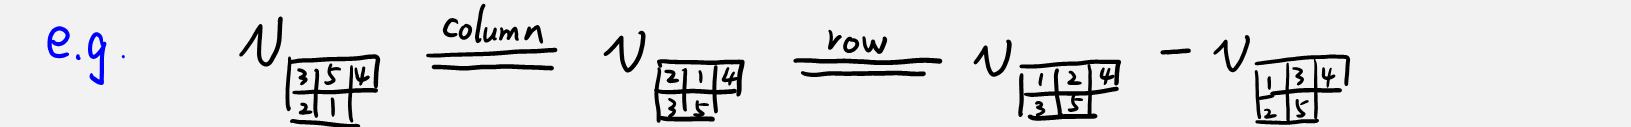
\includegraphics[width=\linewidth]{figure/shadow/eg1.png}
		\item $\left\{  v_{T'} \middle| T': \text{standard tableau} \right\}$ are linear independent.
		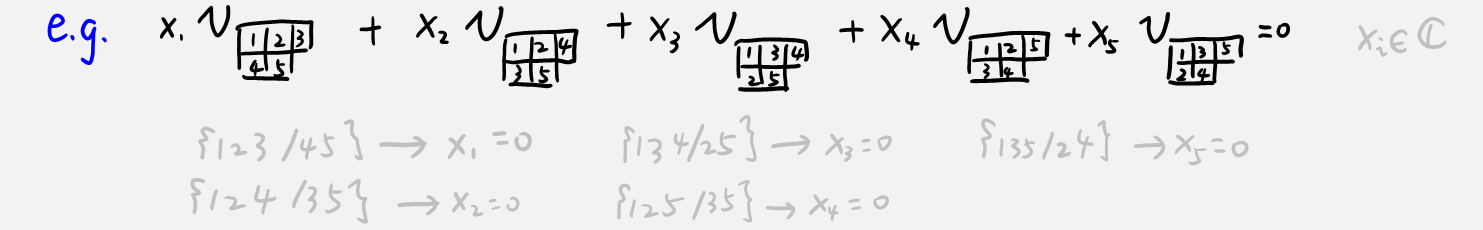
\includegraphics[width=\linewidth]{figure/shadow/eg2.png}
	\end{itemize}
\end{block}
\end{frame}
\begin{frame}{linear ordering}
We use a linear ordering of standard fillings by
		\begin{equation*}
\begin{aligned}
\Young{1&2&3\\4&5}& \longrightarrow 5\, 4\, 3\, 2\, 1\\
\vee\hspace{.6cm} & \\
\Young{1&3&4\\2&5}& \longrightarrow 5\, 2\, 4\, 3\, 1\\
\end{aligned}
\end{equation*}
In the proof, we knock out the biggest one.
%\begin{eg}[(2,2,2) case]
%%			\begin{equation*}
%%	\begin{aligned}
%%	\Young{1&2&3\\4\\5}& > &\Young{1&2&3\\4\\5}& > &\Young{1&2&3\\4\\5}& > &\Young{1&2&3\\4\\5}& > &\Young{1&2&3\\4\\5}& > &\Young{1&2&3\\4\\5} \\[-0.2cm]
%%	\scriptstyle 54321\hspace{0.3cm} &&\scriptstyle 54321\hspace{0.3cm} &&\scriptstyle 54321\hspace{0.3cm} &&\scriptstyle 54321\hspace{0.3cm} &&\scriptstyle 54321\hspace{0.3cm} &&\scriptstyle 54321\hspace{0.3cm}\\
%%	\end{aligned}
%%	\end{equation*}
%				\begin{equation*}
%	\begin{aligned}
%	\Young{1&2\\3&4\\5&6}& >\hspace{-2.5mm} &\Young{1&3\\2&4\\5&6}& >\hspace{-2.5mm} &\Young{1&2\\3&5\\4&6}& >\hspace{-2.5mm} &\Young{1&3\\2&5\\4&6}& >\hspace{-2.5mm} &\Young{1&4\\2&5\\3&6} \\[-0.2cm]
%	\scriptstyle 654321\hspace{0.05cm} &&\scriptstyle 654231\hspace{0.05cm} &&\scriptstyle 645321\hspace{0.05cm} &&\scriptstyle 645231\hspace{0.05cm} &&\scriptstyle 635241\hspace{0.05cm} \\
%	\end{aligned}
%	\end{equation*}
%\end{eg}
\end{frame}
\begin{frame}{Proof: part 2\&3}
\begin{theorem}
	\begin{enumerate}
		\setcounter{enumi}{1}
		\item the representation $S^{\lambda}$ is irreducible;\\
		\item for the Young diagram $\lambda'$, $S^{\lambda'} \cong S^{\lambda} \Rightarrow \lambda'=\lambda$.
	\end{enumerate}
\end{theorem}

\begin{block}{}
	\setlength\abovedisplayskip{1pt plus 3pt minus 7pt}
	\setlength\belowdisplayskip{1pt plus 3pt minus 7pt}
	We have to introduce element $b_T$ in $\mathbb{C}[S_n]$ by  \quad \ignore{fix $T$ of shape $\lambda$}
	$$b_T:=\sum_{q \in C(T)} \sgn (\sigma) \sigma$$
	one can get
 $$b_T  S^{\lambda} =\mathbb{C}  v_T \neq 0,\qquad b_T  S^{\lambda'} = 0 \quad \ignore{\text{ for } \lambda'>\lambda.}\hspace{-1cm}$$
 The results follow from these equations.\quad\hyperlink{skipproof}{\beamergotobutton{skip}}
\end{block}
\end{frame}
\begin{frame}{Proof: part 2\&3}
\begin{theorem}
	\begin{enumerate}
		\setcounter{enumi}{1}
		\item the representation $S^{\lambda}$ is irreducible;\\
		\item for the Young diagram $\lambda'$, $S^{\lambda'} \cong S^{\lambda} \Rightarrow \lambda'=\lambda$.
	\end{enumerate}
\end{theorem}

\begin{block}{}
\setlength\abovedisplayskip{1pt plus 3pt minus 7pt}
\setlength\belowdisplayskip{-5pt plus 3pt minus 7pt}
	We have to introduce element $b_T$ in $\mathbb{C}[S_n]$ by 
	$$b_T:=\sum_{q \in C(T)} \sgn (\sigma) \sigma$$
	then
	\begin{itemize}
		\item $v_T=b_T \cdot \{T\}$;
		\item $\tau(b_T)= \sgn (\tau) b_T \qquad\qquad\qquad$\ignore{for any $\tau \in C(T)$;}
		\item $b_T \cdot b_T= \# C(T) \cdot b_T$;
		\item $b_T  M^{\lambda} = b_T  S^{\lambda} =\mathbb{C}  v_T \neq 0$ ;\\
		$b_T  M^{\lambda'} = b_T  S^{\lambda'} = 0 \qquad\qquad\quad$ \ignore{for $\lambda'>\lambda$.}
	\end{itemize}
\end{block}
\end{frame}
\begin{frame}{Proof: part 2\&3}
 \begin{overlayarea}{\linewidth}{\textheight}
\begin{theorem}
	\begin{enumerate}
		\setcounter{enumi}{1}
		\item the representation $S^{\lambda}$ is irreducible;\\
		\item for the Young diagram $\lambda'$, $S^{\lambda'} \cong S^{\lambda} \Rightarrow \lambda'=\lambda$.
	\end{enumerate}
\end{theorem}

\begin{block}{}
 $\qquad  b_T  S^{\lambda} =\mathbb{C} v_T \neq 0$ ;\\
		$\qquad  b_T  S^{\lambda'} = 0 \qquad\qquad$ for $\lambda'>\lambda$
\end{block}
\only<1>{
\begin{block}{}
	$\divideontimes$To show $S^{\lambda}$ is irreducible: only need to show indecomposablility.\\
	If $S^{\lambda}=V \oplus W$ as $\mathbb{C}[S_n]$-module, then
	\begin{equation*}
	\begin{aligned}
	& \mathbb{C} v_T = b_T  S^{\lambda} =b_T  V \oplus b_T  W\\
	\Rightarrow & b_T  V=\mathbb{C} v_T \qquad\qquad\ignore{\text{(or $b_TW=\mathbb{C} v_T$)}}\\
	\Rightarrow & S^{\lambda}= \mathbb{C}[S_n] \cdot v_T = \mathbb{C}[S_n] \cdot \mathbb{C}v_T = \mathbb{C}[S_n] \cdot b_T V \subseteq V
	\end{aligned}
	\end{equation*}
\end{block}}
\only<2>{
\begin{block}{}
	$\divideontimes$To show $S^{\lambda'} \cong S^{\lambda} \Rightarrow \lambda'=\lambda$:\\
	If not w.l.o.g. suppose $\lambda'>\lambda$. Then
	$$b_TS^{\lambda'}=b_TS^{\lambda} \Longrightarrow \mathbb{C}v_T \cong 0,$$
	contradiction!
\end{block}
}
\end{overlayarea}
\end{frame}
\bgpica{figure/youngdiagram.pdf}
\begin{frame}[label=skipproof]{Example}

\end{frame}
\bgpica{figure/youngdiagramseries.pdf}
\begin{frame}{Example}

\end{frame}
\usebackgroundtemplate{}
\begin{frame}{Example: trivial representation}
 \begin{overlayarea}{\linewidth}{\textheight}

\begin{equation*}
\begin{aligned}
\lambda = & \yng(3)=3^1\\
M^{\lambda} =& \left<\{123 \}\right>=\mathbb{C}\\
T=& \,\Young{1&2&3}\\
C(T)=& \Id\\
v_T=&\left\{123 \right\}\\
S^{\lambda}=&\mathbb{C}[S_3]\cdot v_T =\mathbb{C}v_T\\
\phantom{(2,3)v_T=}&\phantom{\left<\{1/2/3 \},\{1/3/2 \},\{2/1/3 \},\{2/3/1 \},\{3/1/2 \},\{3/2/1 \}\right>_{\mathbb{C}}}\\%强行配平
\end{aligned}
\end{equation*}

\end{overlayarea}
\end{frame}


\begin{frame}{Example: alternating representation}
 \begin{overlayarea}{\linewidth}{\textheight}
	\begin{equation*}
	\begin{aligned}
\lambda = & \yng(1,1,1)=1^3\\
M^{\lambda} =& \left<\{1/2/3 \},\{1/3/2 \},\{2/1/3 \},\{2/3/1 \},\{3/1/2 \},\{3/2/1 \}\right>_{\mathbb{C}}\\
T=& \,\Young{1\\2\\3}\\
C(T)=& S_3\\
v_T=&\{1/2/3\}-\{1/3/2\}-\{2/1/3 \}\\
&\phantom{\{1/2/3\}-\{1/3}+\{2/3/1 \}+\{3/1/2 \}-\{3/2/1 \}\\
S^{\lambda}=&\mathbb{C}[S_3]\cdot v_T =\mathbb{C}v_T\\
\ignore{(23)v_T=}&\ignore{\{1/3/2\}-\{1/2/3\}-\{3/1/2 \}}\\
&\ignore{\phantom{\{1/2/3\}-\{1/3}+\{3/2/1 \}+\{2/1/3 \}-\{2/3/1 \} =-v_T}
	\end{aligned}
	\end{equation*}
\end{overlayarea}
\end{frame}
\begin{frame}{Example: standard representation}
 \begin{overlayarea}{\linewidth}{\textheight}
	\begin{equation*}
\begin{aligned}
\lambda = & \yng(2,1)=2\cdot 1\\
M^{\lambda} =& \left<\{12/3 \},\{13/2 \},\{23/1 \}\right>_{\mathbb{C}}\\
T=& \,\Young{1&2\\3}\\
C(T)=& \left\{\Id, (13)\right\}\\
v_T=&\{12/3\}-\{23/1\}\\
S^{\lambda}=&\mathbb{C}[S_3]\cdot v_T \cong\mathbb{C}^2\\
\ignore{(12)v_T=}&\ignore{\{12/3\}-\{13/2\}}\\
\ignore{(13)v_T=}&\ignore{\{23/1\}-\{12/3\}=-v_T}\\
\phantom{(2,3)v_T=}&\phantom{\left<\{1/2/3 \},\{1/3/2 \},\{2/1/3 \},\{2/3/1 \},\{3/1/2 \},\{3/2/1 \}\right>_{\mathbb{C}}}\\%强行配平
\end{aligned}
\end{equation*}
\end{overlayarea}
\end{frame}
\begin{frame}{Goal \ignore{of the Part 1}}
\begin{itemize}
	\item Explicitly construct irreducible representations of $S_n$ 
	
	by Young diagram;
	\item Compute the character table;
	\begin{itemize}
		\item \stress{$\dim \chi_i$ \hspace{1cm}by recursion} \ignore{/ Hook length formula}
		\item \ignore{character \hspace{.65cm}by Frobenius formula}
	\end{itemize}
	\item \ignore{Compute other representations.}
	\begin{itemize}
		\item \ignore{e.g. $\otimes,\, \Sym^m,\, \Lambda^m$;}
		\item \ignore{e.g. $M_{\lambda}$.}
		\item \ignore{restriction and induced representation}
			\item \ignore{representation ring}
	\end{itemize}
\end{itemize}
\end{frame}
\begin{frame}[fragile]{Example: dimension of irreducible representation}
\begin{overlayarea}{\linewidth}{\textheight}
$$\dim S^{\lambda}=\#\{ \text{standard tableau of } \lambda \} =\,\, ?$$

\begin{eg}
	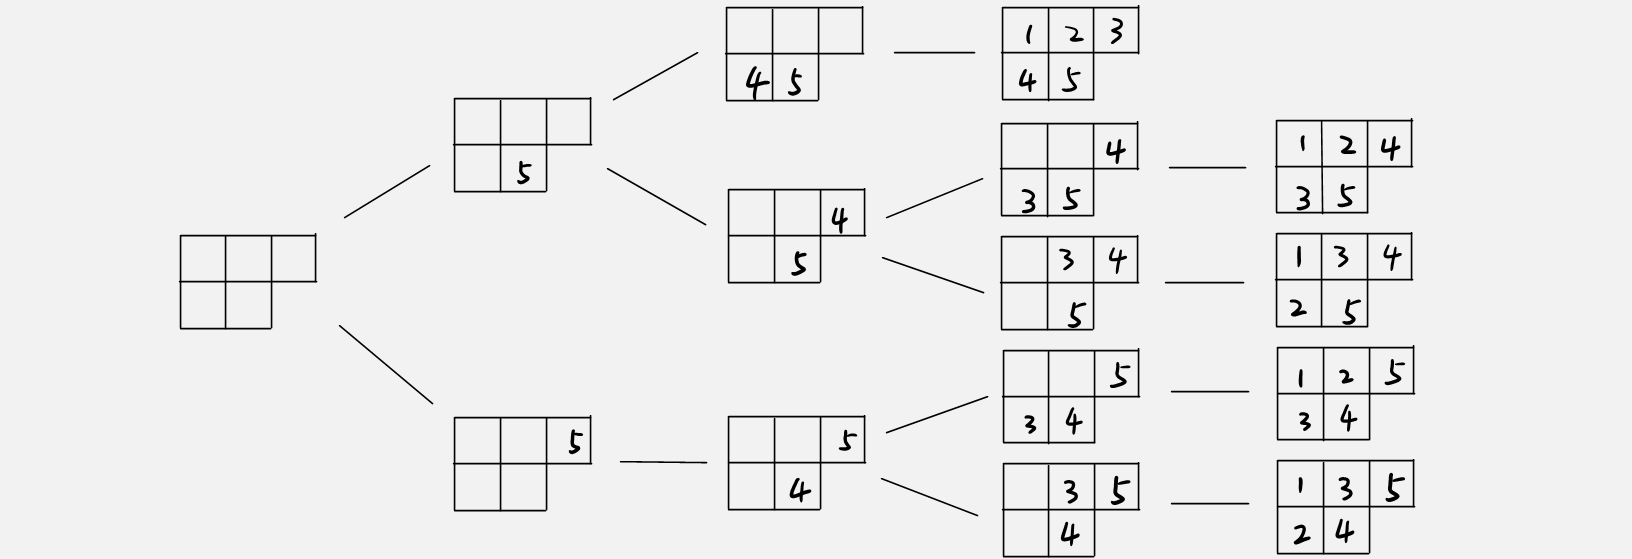
\includegraphics[width=\linewidth]{figure/shadow/induction.png}
%	$\Young{1&2}$
%	\begin{tikzcd}
%		\Young{1&2}
%	\end{tikzcd}
%% https://tikzcd.yichuanshen.de/#N4Igdg9gJgpgziAXAbVABwnAlgFyxMJZABgBoAmAXVJADcBDAGwFcYkQAdDgTQmbADmwAGTCuXYQF8Qk0uky58hFAEZSK6nSat2XXvyGjxHYQFZps+djwEiagMyaGLNok48+gkWeNSZckAxrJSJyUgAWJ21Xd30vUVNfcIsAoMVbFDDiKJddDwNvY3CzFKt05WQwqhpnHTc9T0NhcN9zfzKbCvtSbJrovLihFWFyYXsikvbAhU6ibo0+3Pr8+Obje0nLaeCM5G7qrSXYxpENlvFN1JmQlG7HRbrjgoT15tLt8rmInMeG543EhdklM0rMUOF1D8Yn8vMNRucuAD3qCbsgIQdatCVkMxmtxKM2lsUbsIfdDr9scA4T5xGdkdcSd8HljBlTcYCuPCLJoYFABPAiKAAGYAJwgAFskGQQDgIEg1CAABYwehQdiQMBsLaiiVSmiypBhJUqtVuDVagI6yWII0GxDdY2q9UEC3CsXWhV2iGO03gF1TK3y-VyxCmGjKp1m-3a91Ib12gBs4ZNzs1AdjoeDSAA7MnI360zHdZmZSGABx533m9PFh12gCcldTrpAgftWcQKmlEar0ctGdzpflCp7zZr1orQ87RtHUcL-eLjanKgds4LLbbXY7Km9a+rkkokiAA
%\begin{tikzcd}
%	&                                                        & \Young{&&\\4&5} \arrow[r, no head]                     & \Young{1&2&3\\4&5}                  &                    \\
%	& \Young{&&\\&5} \arrow[ru, no head] \arrow[rd, no head] &                                                        & \Young{&&4\\3&5} \arrow[r, no head] & \Young{1&2&4\\3&5} \\
%	\Young{&&\\&} \arrow[ru, no head] \arrow[rd, no head] &                                                        & \Young{&&4\\&5} \arrow[ru, no head] \arrow[r, no head] & \Young{&3&4\\&5} \arrow[r, no head] & \Young{1&3&4\\2&5} \\
%	& \Young{&&5\\&} \arrow[rd, no head]                     &                                                        & \Young{&&5\\3&4} \arrow[r, no head] & \Young{1&2&5\\3&4} \\
%	&                                                        & \Young{&&5\\&4} \arrow[ru, no head] \arrow[r, no head] & \Young{&3&5\\&4} \arrow[r, no head] & \Young{1&3&5\\2&4}
%\end{tikzcd}
\end{eg}
\only<2>{\vspace{-0.3cm}
$$\dim S^{\lambda}=\sum_{\substack{\lambda' \subseteq \lambda\\ |\lambda'|=n-1}} \dim S^{\lambda'}$$}
\end{overlayarea}
\end{frame}
\bgpicb{figure/youngdiagram.pdf}
\begin{frame}{Example: dimension of irreducible representation}


\end{frame}
\bgpicb{figure/youngdiagram1.pdf}
\begin{frame}{Example: dimension of irreducible representation}


\end{frame}
\usebackgroundtemplate{}
\begin{frame}[fragile]{Hook length formula}
% \begin{overlayarea}{\linewidth}{\textheight}
It helps us compute the dimension of $S^{\lambda}$ without induction.

Step 1: count the length of hook.
$$\setlength{\Youngwidth}{2pc}\setlength{\Youngheight}{2pc}
\def\Fontinbox#1{\setlength{\Youngwidth}{0.5pc}\setlength{\Youngheight}{0.5pc}{#1}}
\young{\young{\hook[dr]&\hook[lr]&\hook[l]\\\hook[u]}&
	\young{&\hook[r]&\hook[l]\\}&
	\young{&&\hook[c]\\}\\
	\young{&&\\\hook[c]}
} \quad\raisebox{7mm}{$\Longrightarrow$}\quad \young{\raisebox{1mm}{$4$}&\raisebox{1mm}{$2$}&\raisebox{1mm}{$1$}\\\raisebox{1mm}{$1$}}$$
Step 2: $\displaystyle \dim S^{\lambda} = \frac{n!}{\prod (\text{hook lengths})}$
%\end{overlayarea}

\end{frame}
\begin{frame}[fragile]{Special case: $(m,l)$}
\begin{overlayarea}{\linewidth}{\textheight}
\begin{block}{Ballot problem}
	In an election where candidate A receives $m$ votes and candidate B receives $l$ votes with $m \geqslant l$, what is the probability that A will be (non-strictly) ahead of B throughout the count?
\end{block}
\begin{proposition}
	Each process of the count corresponds to each standard tableau of form $(m,l)$.
\end{proposition}
\begin{eg}
	\hspace{3cm}\raisebox{1cm}{$\Young{1&3&4\\2&5} \longleftrightarrow$} 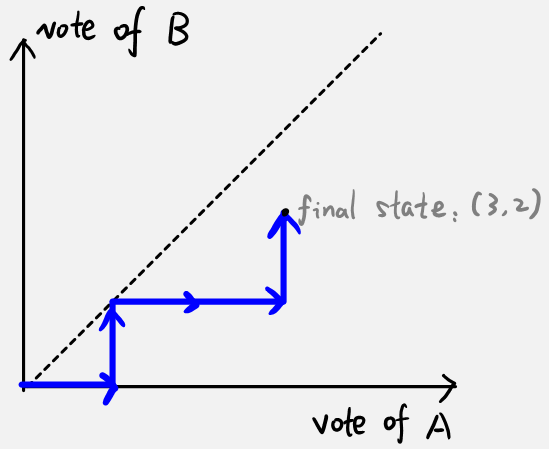
\includegraphics[width=2.5cm]{figure/shadow/vote.png}
\end{eg}

\end{overlayarea}
\end{frame}
\begin{frame}[fragile]{Special case: $(m,m)$}
\begin{overlayarea}{\linewidth}{\textheight}
	\vspace{-0.5cm}
\begin{cor}
	 $$\dim S^{(m,m)}= C_m = \frac{1}{m+1} \binom{2m}{m}.$$
	 where $C_m$ is the $m$-th Catalan number.
\end{cor}
		\only<2-3>{Catalan number has many interpretations. For example, it counts the number of crossingless matchings of $2m$ points.}
		\only<2>{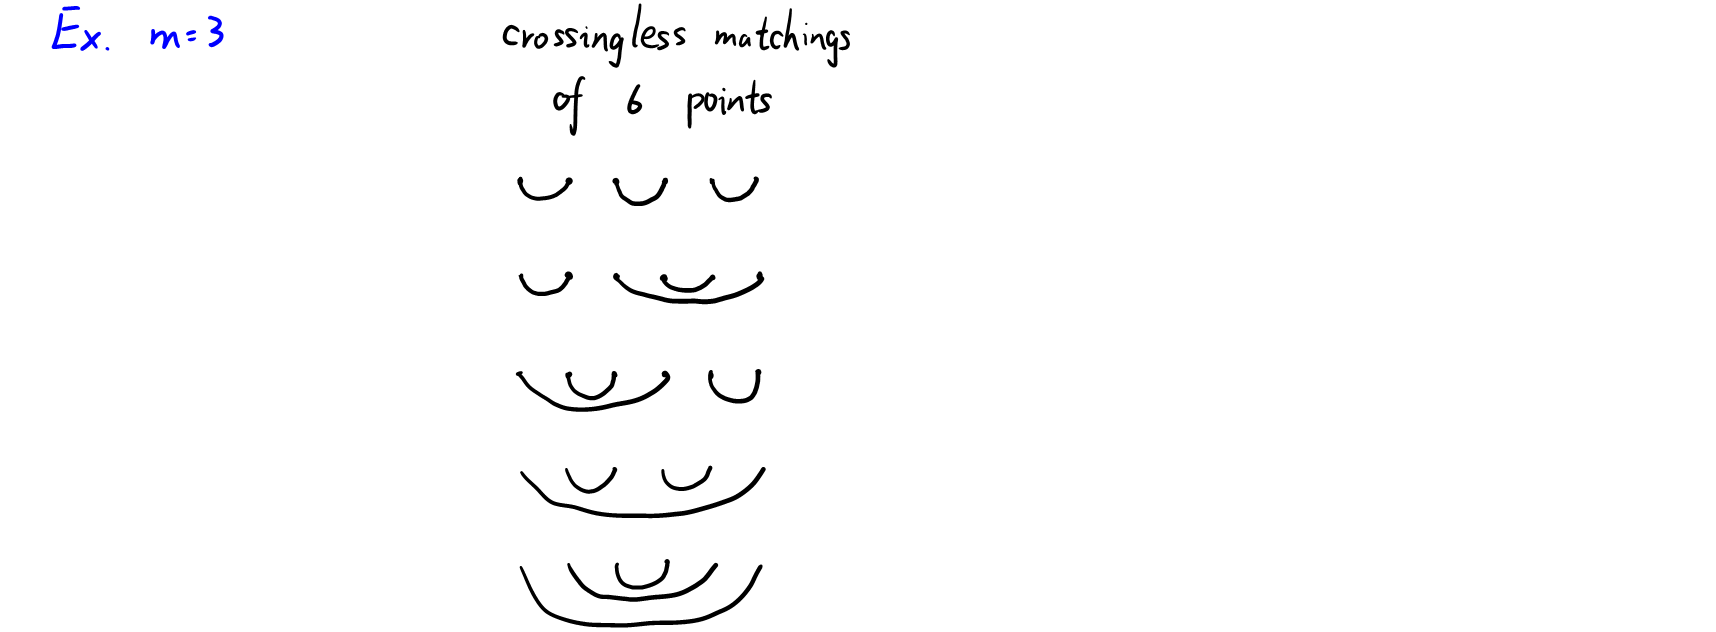
\includegraphics[width=\linewidth]{figure/shadow/crossingless2.png}}
		\only<3>{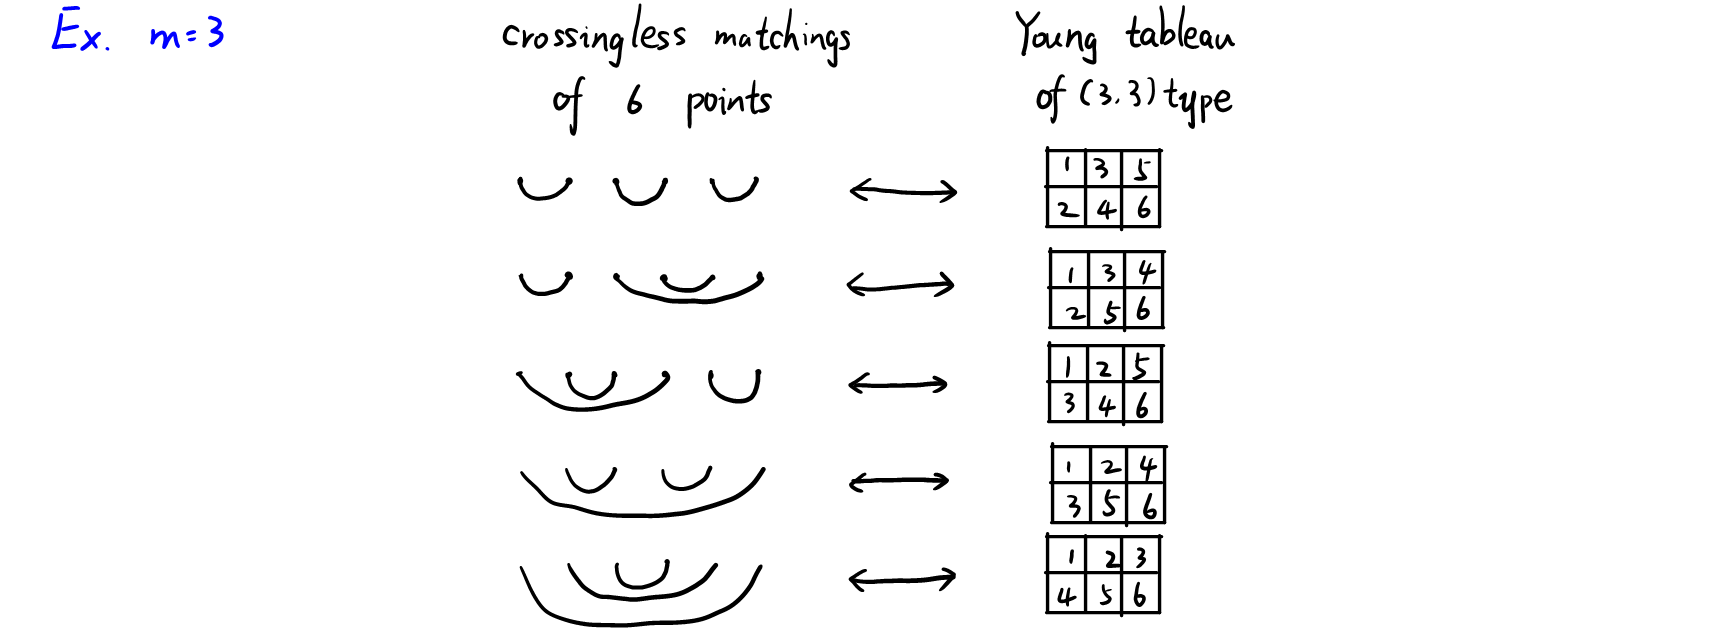
\includegraphics[width=\linewidth]{figure/shadow/crossingless.png}}
\end{overlayarea}
\end{frame}

%%%%%%%%%Part II


\begin{frame}{Goal \ignore{of the Part II}}
\begin{itemize}
	\item Definition of Springer fiber;
	\item Some examples of Springer fiber;
	\item Properties: \ignore{(closely connected with combinatorics)}
	\begin{itemize}
		\item irreducible component?
		\item dimension?
		\item affine paving? -- CW complex?
		\item cohomology? -- ring structure?
		\item smooth?
		\item explicit description?%\ignore{local chart, fiber bundle}
	\end{itemize}
\item \ignore{Weyl group action on top homology}.
\end{itemize}
\end{frame}
\begin{frame}{Goal \ignore{of the Part II}}
\begin{itemize}
	\item \stress{Definition} of Springer fiber;
	\item Some examples of Springer fiber;
	\item Properties: \ignore{(closely connected with combinatorics)}
	\begin{itemize}
		\item irreducible component?
		\item dimension?
		\item affine paving? -- CW complex?
		\item cohomology? -- ring structure?
		\item smooth?
		\item explicit description?%\ignore{local chart, fiber bundle}
	\end{itemize}
	\item \ignore{Weyl group action on top homology}.
\end{itemize}
\end{frame}
\begin{frame}
	\begin{defn}
		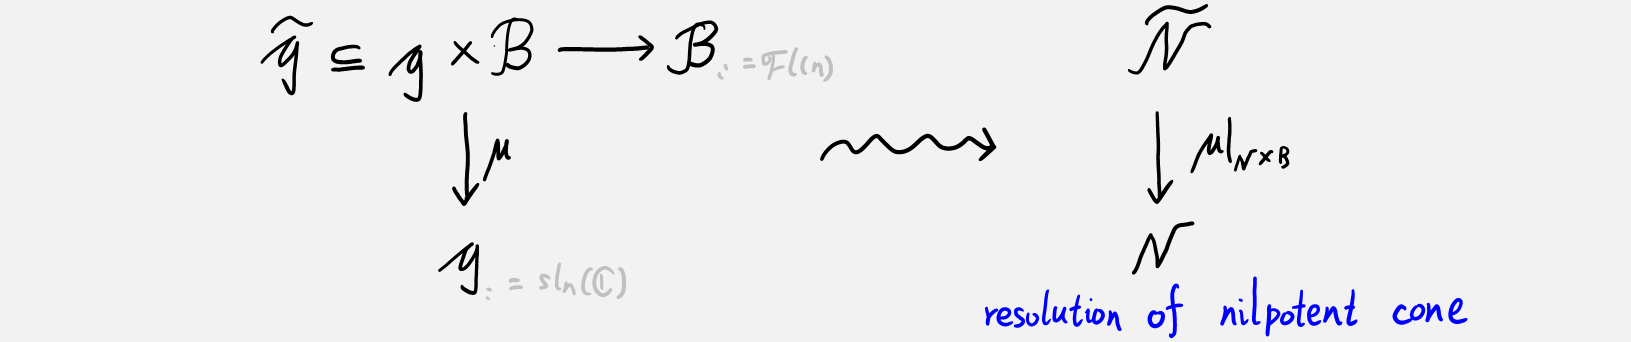
\includegraphics[width=\linewidth]{figure/shadow/defspringer.png}
		Let $X \in \mathfrak{g}$ be a nilpotent element. The Springer fiber $B_X$ over $X$ is defined as
		\begin{equation*}
		\begin{aligned}
		B_X:= & \mu^{-1}(X) \\
		= & \{B \in \mathfrak{B} \mid X \in B  \}\\
		= & \left\{ 0 \subseteq V_1 \subseteq V_2\subseteq \cdots\subseteq V_n=\mathbb{C}^n \middle| XV_i \subseteq V_{i-1}  \right\} \;\ignore{\dim V_i=i}
		\end{aligned}
		\end{equation*}
	\end{defn}
\end{frame}

\begin{frame}
 \begin{overlayarea}{\linewidth}{\textheight}
\begin{block}{}
	By the Jordan normal form, we have
	$$\left\{ \begin{gathered}
	\text{Nilpotent element}\\\text{in $\mathfrak{gl}_n(\mathbb{C})$}
	\end{gathered}  \right\}_{\Big/\text{conj}}\xleftrightarrow{\quad\quad}\qquad\left\{ \begin{gathered}
	\text{Young diagram}\\\text{of $n$ boxes}
	\end{gathered}  \right\} $$
	$$\hspace{-0.5cm}X_{\lambda}=\diag(\underbrace{J_{\lambda_1},\ldots,J_{\lambda_1}}_{v_1},J_{\lambda_2},\ldots,J_{\lambda_k}) \hspace{.3cm}\xleftrightarrow{\quad\quad}\hspace{.3cm} \lambda=\lambda_1^{v_1} \cdots \lambda_k^{v_k}$$
\end{block}

	
Denote $B_{\lambda}:=B_{X_{\lambda}}$. \qquad \ignore{$B_X \cong B_{gXg^{-1}}$ for any $g \in G$}

\begin{theorem}[we will not give the proof.]
	As $S_n$-representation, $S^{\lambda}\cong H_{\text{top}}(B_{\lambda})$.
\end{theorem}
\begin{cor}
	 $\#\{\text{irreducible component of } B_{\lambda}\} = \dim S^{\lambda}$
\end{cor}
\end{overlayarea}
\end{frame}

\begin{frame}{Goal \ignore{of the Part II}}
\begin{itemize}
	\item Definition of Springer fiber;
	\item Some \stress{examples} of Springer fiber;
	\item \stress{Properties}: \ignore{(closely connected with combinatorics)}
	\begin{itemize}
		\item irreducible component?
		\item dimension?
		\item affine paving? -- CW complex?
		\item cohomology? -- ring structure?
		\item smooth?
		\item explicit description?%\ignore{local chart, fiber bundle}
	\end{itemize}
	\item \ignore{Weyl group action on top homology}.
\end{itemize}
\end{frame}

\bgpica{figure/youngdiagramseries.pdf}
\begin{frame}{tree of Young diagram}

\end{frame}
\usebackgroundtemplate{}
\begin{frame}{Example: $\lambda=3 \quad \Yng(3)$}
\begin{overlayarea}{\linewidth}{\textheight}
	
	\begin{equation*}
	\begin{aligned}
	X_{\lambda}=&\begin{bmatrix}
	0 & 1 & \\
	  & 0 & 1 \\
	  &   & 0
	\end{bmatrix}\\
	B_{\lambda}= & \left\{ 0 \subseteq \left<\ques\right>\subseteq \left<\ques,\ques\right> \subseteq \mathbb{C}^3 \right\} \ignore{\curvearrowleft X_{\lambda}} \quad=\{*\}\\
	\end{aligned}
	\end{equation*}
	In general, $B_{\lambda}=\{*\}$ when $\lambda$ has only one row.
\end{overlayarea}
\end{frame}
\begin{frame}{Example: $\lambda=(1,1,1) \quad \Yng(1,1,1)$}
\begin{overlayarea}{\linewidth}{\textheight}
	
	\begin{equation*}
	\begin{aligned}
	X_{\lambda}=&\begin{bmatrix}
	0 &  & \\
	& 0 &  \\
	&   & 0
	\end{bmatrix}\\
	B_{\lambda}= & \left\{ 0 \subseteq \left<\ques\right>\subseteq \left<\ques,\ques\right> \subseteq \mathbb{C}^3 \right\} \ignore{\curvearrowleft X_{\lambda}} \quad=\Fl(3)\\
	\end{aligned}
	\end{equation*}
	In general, $B_{\lambda}=\Fl(n)$ when $\lambda=1^n$.
\end{overlayarea}
\end{frame}
\begin{frame}{Properties of $B_{\lambda}=\Fl(n)$}
	\begin{itemize}
		\item irreducible:
		\item $\dim B_{\lambda}=$
		\item CW complex:
		\item cohomology group:
		\item smooth:
		\item explicit description:
		\item Weyl group action on $H_{\text{top}}(B_{\lambda})\cong \mathbb{C}$:
	\end{itemize}


\end{frame}
\begin{frame}{Example: $\lambda=(2,1) \quad \Yng(2,1)$}
\begin{overlayarea}{\linewidth}{\textheight}
	
	\begin{equation*}
	\begin{aligned}
	X_{\lambda}=&\begin{bmatrix}
	0 & 1 & \\
	& 0 &  \\
	&   & 0
	\end{bmatrix}\\
	B_{\lambda}= & \left\{ 0 \subseteq \left<\ques\right>\subseteq \left<\ques,\ques\right> \subseteq \mathbb{C}^3 \right\} \ignore{\curvearrowleft X_{\lambda}} \quad=\mathbb{P}^1 \vee \mathbb{P}^1\\
	\end{aligned}
	\end{equation*}
\begin{block}{}
	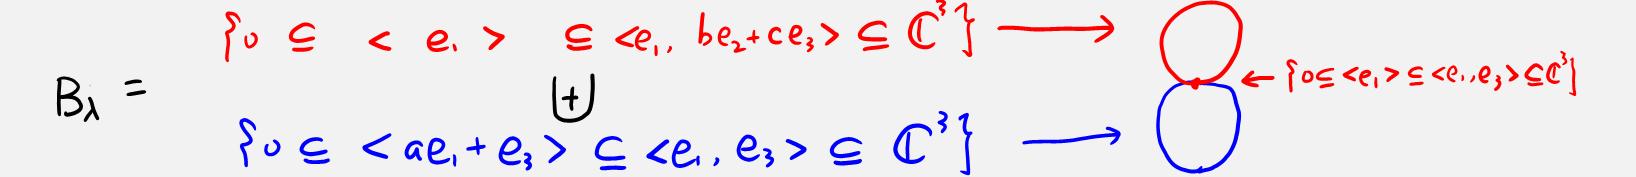
\includegraphics[width=\linewidth]{figure/shadow/case(2,1).png}
\end{block}
	In general, $B_{\lambda}=\underbrace{\mathbb{P}^1 \vee\cdots\vee \mathbb{P}^1}_{n-1}$ when $\lambda=(n-1,1)$.
\end{overlayarea}
\end{frame}
\begin{frame}{Properties of $B_{\lambda}=\underbrace{\mathbb{P}^1 \vee\cdots\vee \mathbb{P}^1}_{n-1}$}
\begin{itemize}
	\item irreducible component:
	\item $\dim B_{\lambda}=$
	\item affine paving:
	\item cohomology group:
	\item smooth:
	\item explicit description:
	\item Weyl group action on $H_{\text{top}}(B_{\lambda}) \cong \mathbb{C}^{n-1}$:
\end{itemize}


\end{frame}
\begin{frame}{Tool: stratification/cellular fibration/affine paving}
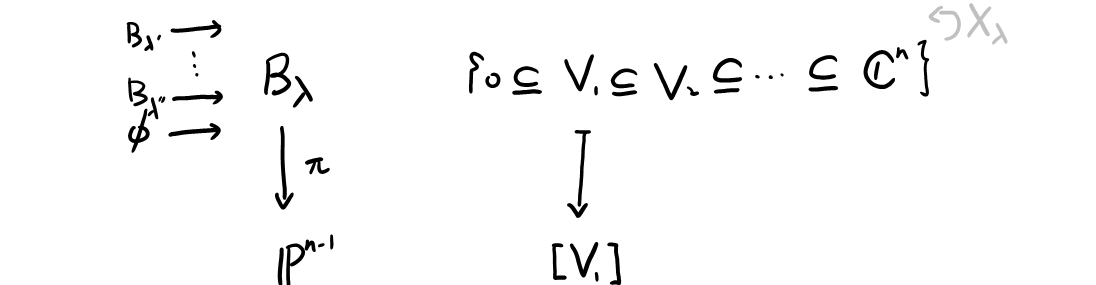
\includegraphics[width=\linewidth]{figure/shadow/myidea.png}
\begin{remark}
	In general, we don't understand the ring structure of the cohomology group.
\end{remark} 
\end{frame}
\begin{frame}[fragile]{Return!}
\begin{overlayarea}{\linewidth}{\textheight}
	For $\lambda=1^3$, $B_{\lambda} \cong \Fl(3)$ can be viewed as $\Fl(2)$-bundle over $\mathbb{P}^2$.
	\begin{figure}[h]
		\centering
	\begin{tikzcd}
	\Fl(2) \arrow[r] & \Fl(3) \arrow[d, "\pi", two heads] \\
	& \mathbb{P}^2                      
\end{tikzcd}
	\end{figure}

	$$\pi^{-1}([v])=\left\{ 0 \subseteq \left<v\right> \subseteq \left<v, \ques\right> \subseteq \mathbb{C}^3 \right\} \cong \Fl(2)$$
\end{overlayarea}
\end{frame}
\begin{frame}[fragile]{Return!}
\begin{overlayarea}{\linewidth}{\textheight}
	For $\lambda=(2,1)$, $B_{\lambda} \cong \mathbb{P}^1 \vee \mathbb{P}^1$: 
%			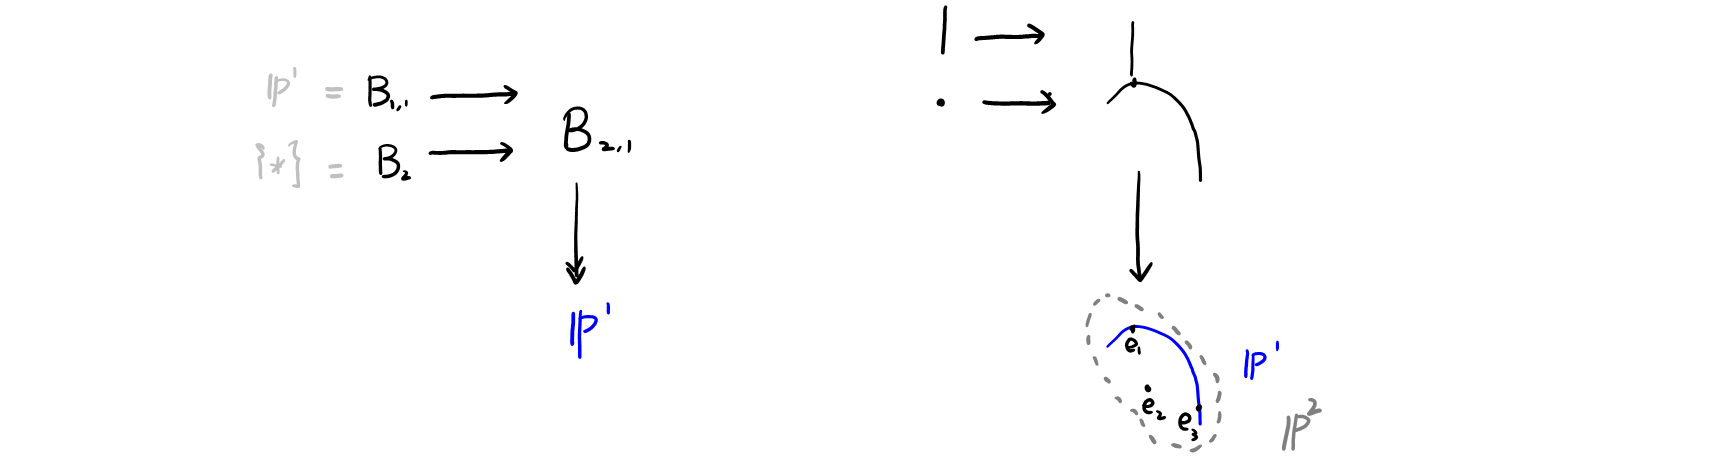
\includegraphics[width=\linewidth]{figure/shadow/case(2,1)new.png}
\only<1,2>{			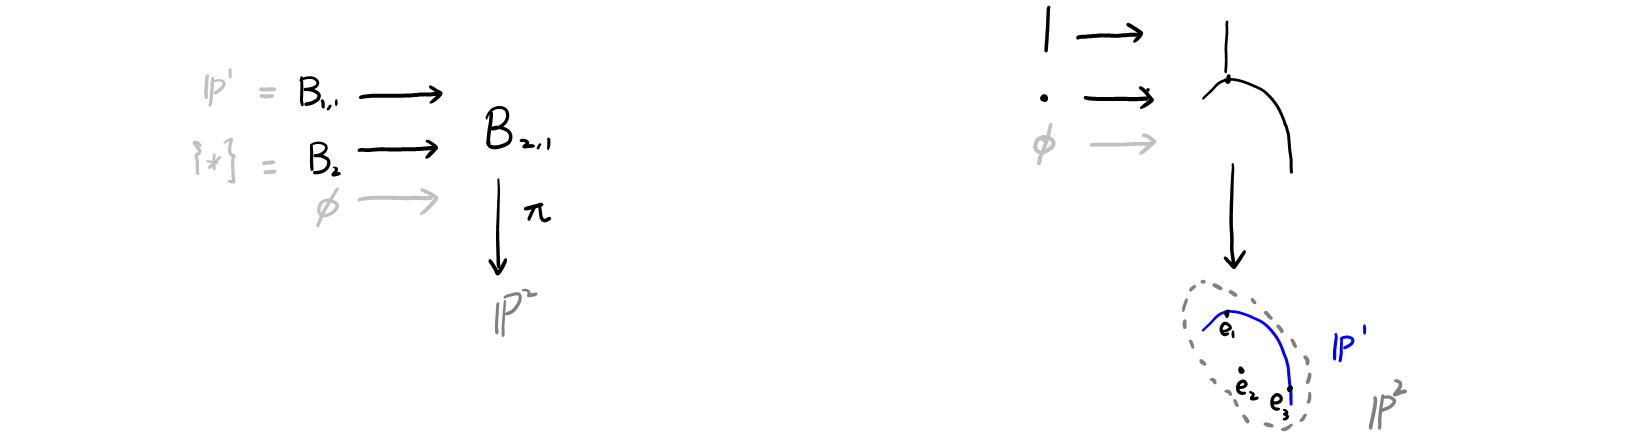
\includegraphics[width=\linewidth]{figure/shadow/case(2,1)series1.png}
}
\only<3>{			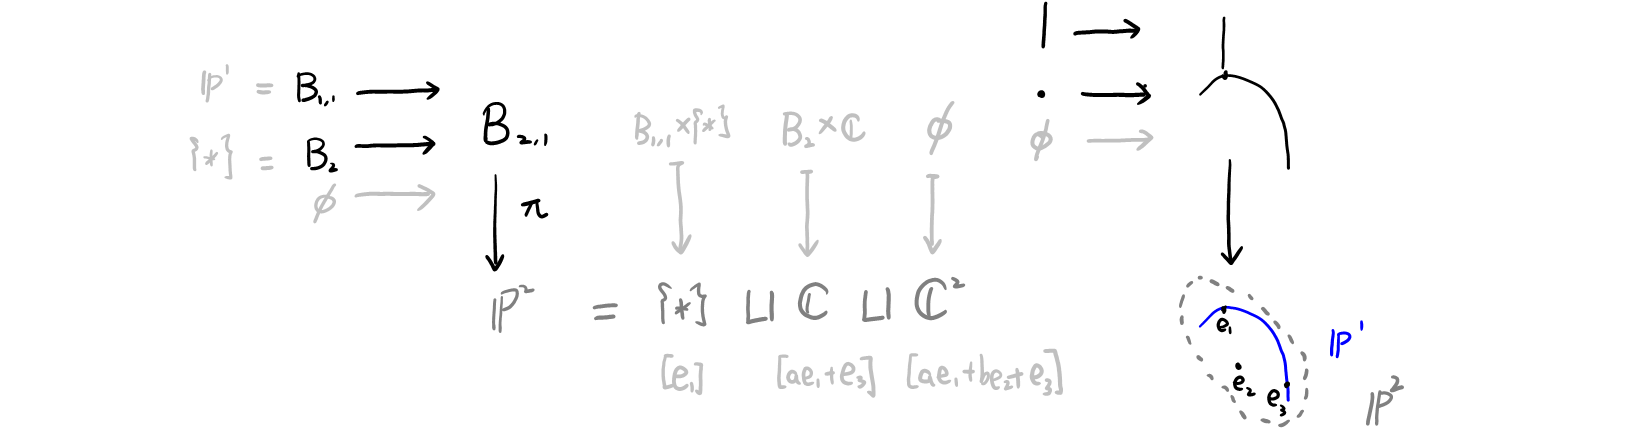
\includegraphics[width=\linewidth]{figure/shadow/case(2,1)series2.png}
}
\only<4>{			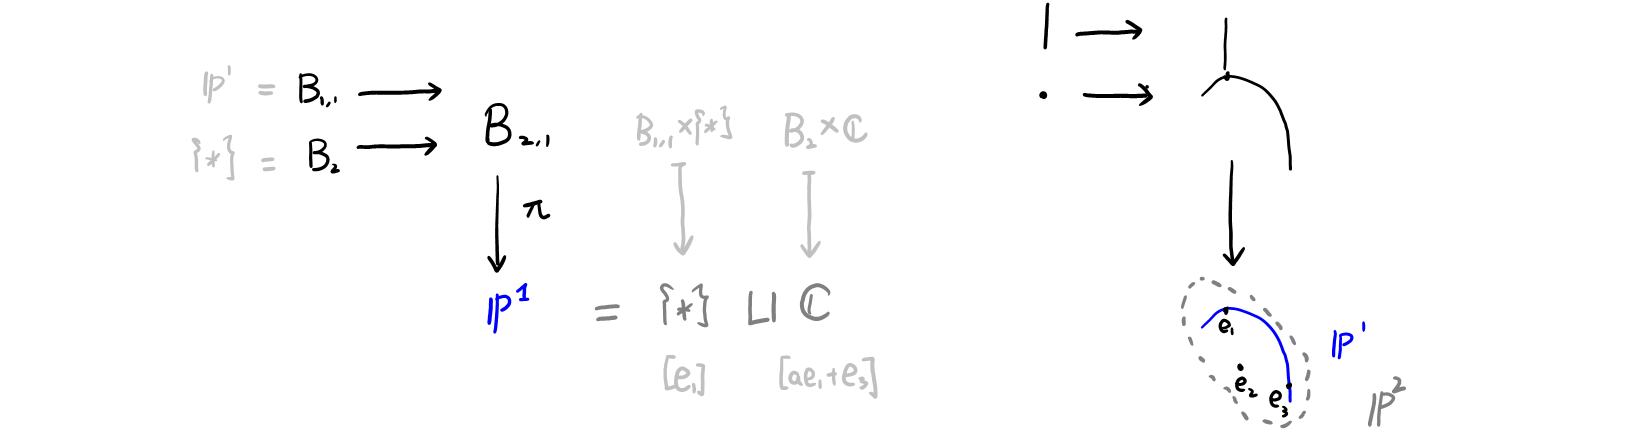
\includegraphics[width=\linewidth]{figure/shadow/case(2,1)series3.png}
}
\only<1>{
			\begin{equation*}
			\begin{aligned}
				\pi^{-1}([e_1])=&\left\{ 0 \subseteq \left<e_1\right> \subseteq \left<\ques, \ques\right> \subseteq \mathbb{C}^3 \right\} \ignore{\curvearrowleft \left[\begin{smallmatrix}
					0 & 1 & \\ & 0 & \\ & & 0
					\end{smallmatrix}\right]}&& \\
				\cong & \left\{ 0 \subseteq \left<\ques\right> \subseteq  \mathbb{C}^2 \right\} \ignore{\curvearrowleft \left[\begin{smallmatrix}
					0 &  \\ & 0
					\end{smallmatrix}\right]}&& = B_{1,1}\\
				\pi^{-1}([e_3])=&\left\{ 0 \subseteq \left<e_3\right> \subseteq \left<\ques, \ques\right> \subseteq \mathbb{C}^3 \right\} \ignore{\curvearrowleft \left[\begin{smallmatrix}
					0 & 1 & \\ & 0 & \\ & & 0
					\end{smallmatrix}\right]}&& \\
				\cong & \left\{ 0 \subseteq \left<\ques\right> \subseteq  \mathbb{C}^2 \right\} \ignore{\curvearrowleft \left[\begin{smallmatrix}
					0 & 1 \\ & 0
					\end{smallmatrix}\right]}&& =  B_{2}\\
				\pi^{-1}([e_2]) =&\left\{ 0 \subseteq \left<e_2\right> \subseteq \left<\ques, \ques\right> \subseteq \mathbb{C}^3 \right\} \ignore{\curvearrowleft \left[\begin{smallmatrix}
					0 & 1 & \\ & 0 & \\ & & 0
					\end{smallmatrix}\right]} && = \varnothing \\
			\end{aligned}
			\end{equation*}
}
\only<2-4>{
	$$\pi^{-1}([e_1])\cong B_{1,1} \qquad \pi^{-1}([e_3])\cong B_{2}\qquad \pi^{-1}([e_2])\cong \varnothing$$
\only<3-4>{				\begin{equation*}
	\begin{aligned}
	\pi^{-1}([ae_1+e_3])=&\left\{ 0 \subseteq \left<ae_1+e_3\right> \subseteq \left<\ques, \ques\right> \subseteq \mathbb{C}^3 \right\} \ignore{\curvearrowleft \left[\begin{smallmatrix}
		0 & 1 & \\ & 0 & \\ & & 0
		\end{smallmatrix}\right]} \\
	\cong & \left\{ 0 \subseteq \left<f_3\right> \subseteq \left<\ques, \ques\right> \subseteq \mathbb{C}^3 \right\} \ignore{\curvearrowleft \left[\begin{smallmatrix}
		0 & 1 & \\ & 0 & \\ & & 0
		\end{smallmatrix}\right]} \\
	\end{aligned}
	\end{equation*}
%By this way, $\pi^{-1}(\mathbb{P}^1 \setminus \{[e_1] \}) \cong B_2 \times \mathbb{C}$ induces an affine paving.
}
}
\end{overlayarea}
\end{frame}
\begin{frame}{Example: $\lambda=(2,1,1) \quad \Yng(2,1,1)$}
\begin{overlayarea}{\linewidth}{\textheight}
	
	\begin{equation*}
	\begin{aligned}
	X_{\lambda}=&\begin{bmatrix}
	0 & 1 & & \\
	& 0 & & \\
	&   & 0 & \\
	& & & 0
	\end{bmatrix}\\
	B_{\lambda}= & \left\{ 0 \subseteq \left<\ques\right>\subseteq \left<\ques,\ques\right> \subseteq \left<\ques,\ques,\ques\right> \subseteq \mathbb{C}^4 \right\} \ignore{\curvearrowleft X_{\lambda}}\\
	\end{aligned}
	\end{equation*}
			\only<1>{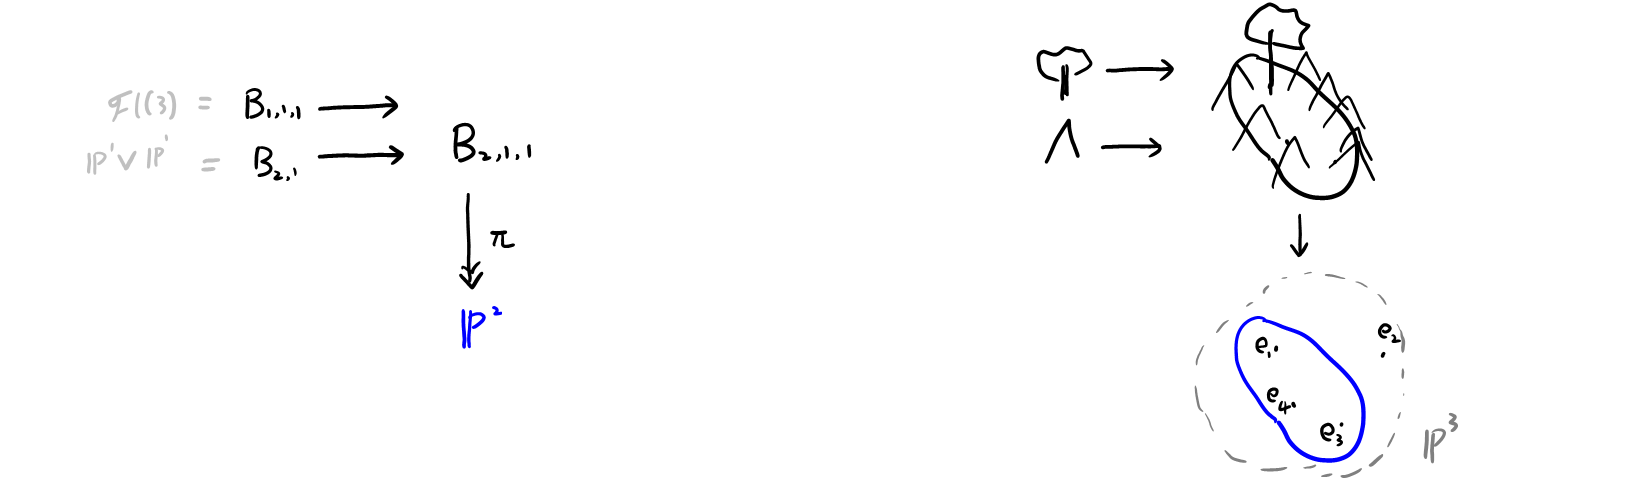
\includegraphics[width=\linewidth]{figure/shadow/case(2,1,1)del.png}}
\only<2>{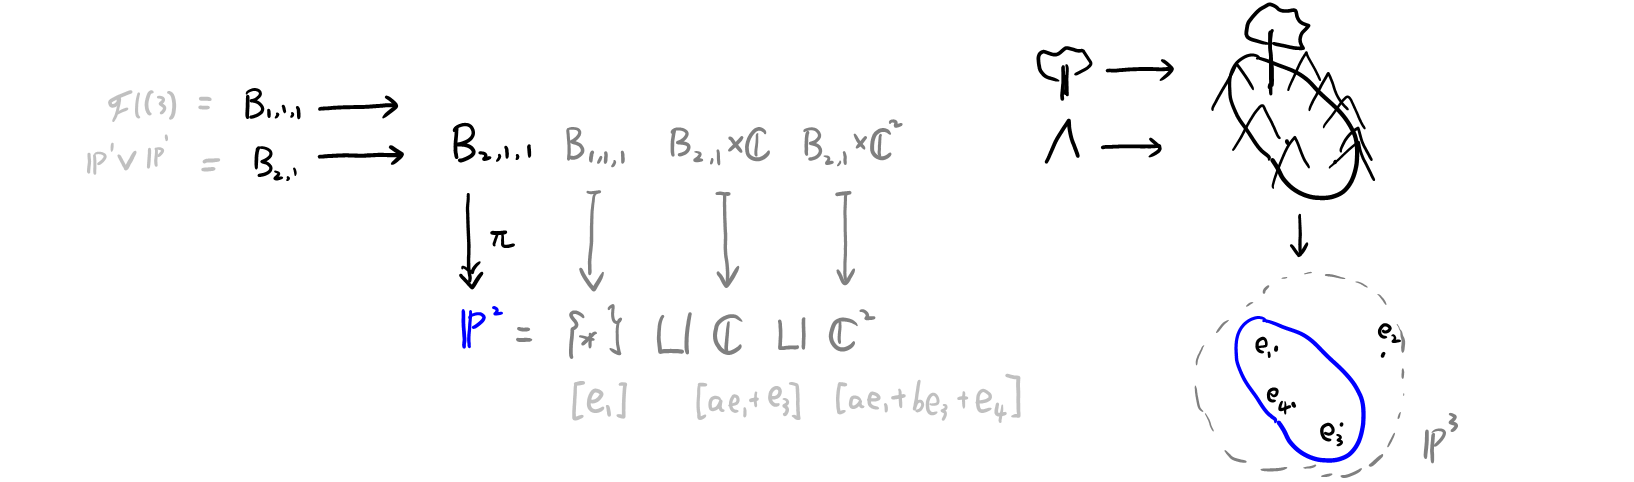
\includegraphics[width=\linewidth]{figure/shadow/case(2,1,1).png}}
\end{overlayarea}
\end{frame}
\begin{frame}{Example: $\lambda=(2,2) \quad \Yng(2,2)$}
\begin{overlayarea}{\linewidth}{\textheight}
	
	\begin{equation*}
	\begin{aligned}
	X_{\lambda}=&\begin{bmatrix}
	0 & 1 & & \\
	& 0 & & \\
	&   & 0 & 1 \\
	& & & 0
	\end{bmatrix}\\
	B_{\lambda}= & \left\{ 0 \subseteq \left<\ques\right>\subseteq \left<\ques,\ques\right> \subseteq \left<\ques,\ques,\ques\right> \subseteq \mathbb{C}^4 \right\} \ignore{\curvearrowleft X_{\lambda}}\\
	\end{aligned}
	\end{equation*}
			\only<1>{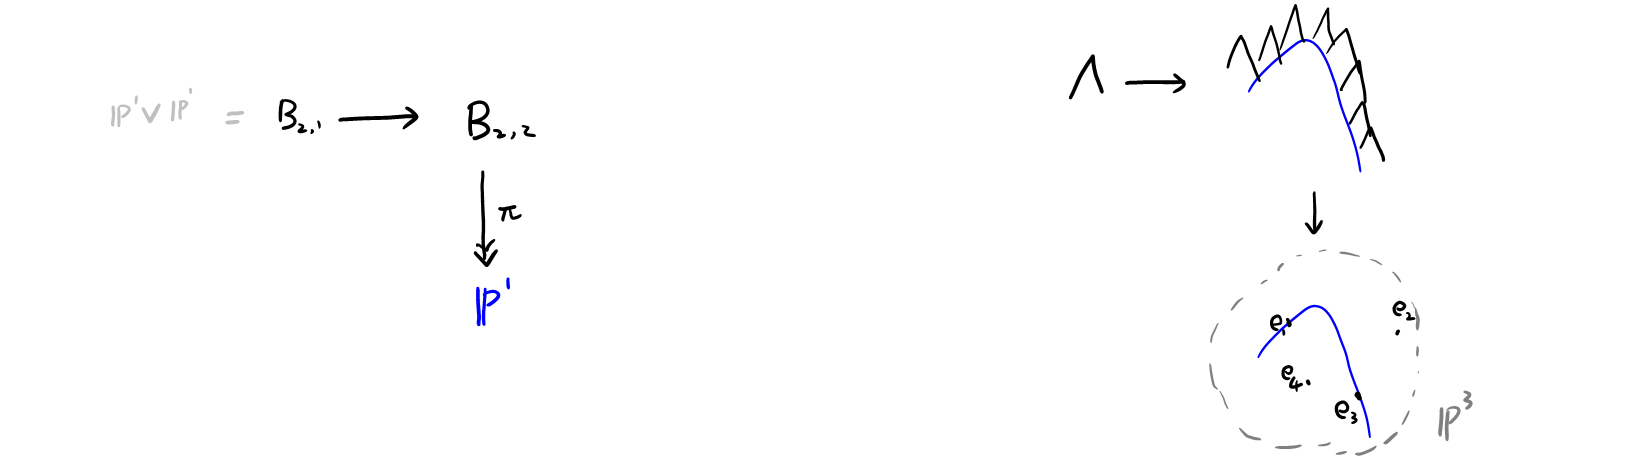
\includegraphics[width=\linewidth]{figure/shadow/case(2,2)del.png}}
			\only<2>{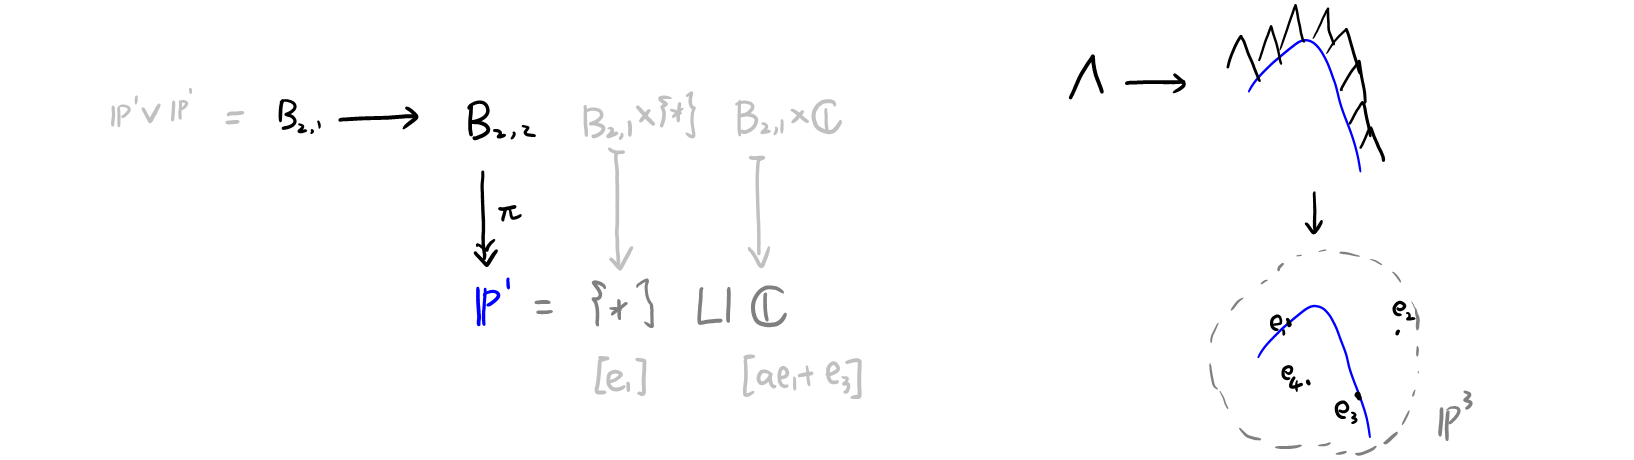
\includegraphics[width=\linewidth]{figure/shadow/case(2,2).png}}
\end{overlayarea}
\end{frame}
\begin{frame}
	Using the same technique, we can get
	\begin{itemize}
		\item $B_{\lambda}$ has an affine paving $\rightsquigarrow$ cohomology;
		\item Each irreducible component in $B_{\lambda}$ has same dimension;
		\item It's easy to compute the dimension and the number of irreducible component.
	\end{itemize}
\end{frame}
\bgpicb{figure/youngdiagram0.pdf}
\begin{frame}{Game: compute!}

\end{frame}
\bgpicb{figure/youngdiagram2.pdf}
\begin{frame}{Answer: dimension }

\end{frame}
\bgpicb{figure/youngdiagram1.pdf}
\begin{frame}{Answer: the number of irreducible component}

\end{frame}

\usebackgroundtemplate{}
\begin{frame}{Smooth problem}
	\begin{block}{Results}
			\setlength\abovedisplayskip{1pt plus 3pt minus 7pt}
		\setlength\belowdisplayskip{1pt plus 3pt minus 7pt}
		\begin{itemize}
			\item Not all the the irreducible components of $B_{\lambda}$ are smooth;\\
			For example, one component of $B_{2,2,1,1}$ is not smooth.\\
			\item All the components of $B_{\lambda}$ are nonsingular iff 
			$$\lambda \in \{(\lambda_1,1,1,\ldots),(\lambda_1,\lambda_2),(\lambda_1,\lambda_2,1),(2,2,2)\}$$
		\end{itemize}
		
	\end{block}
\end{frame}
\bgpicb{figure/youngdiagram0.pdf}
\begin{frame}{tree of Young diagram}

\end{frame}
\usebackgroundtemplate{}
\begin{frame}{$(m,m)$ case}
	\only<1>{We have an explicit description in the 2-row case when we forget the variety structure. Use this description, we can get the cohomology group structure.}
\begin{block}{Definition and Theorem}
	\setlength\abovedisplayskip{1pt plus 3pt minus 7pt}
	\setlength\belowdisplayskip{1pt plus 3pt minus 7pt}
	Let $\alpha$ be a crossingless matching, define
\begin{equation*}
\begin{aligned}
\tilde{B}_{\alpha;\,m,m}:= & \left\{(x_1,\ldots,x_{2m}) \in (\mathbb{P}^1)^{2m} \middle| x_i =x_j \text{ if }(i,j) \in \alpha   \right\} \ignore{\subseteq (\mathbb{P}^1)^{2m}}\\
\tilde{B}_{m,m}:= & \bigcup_{\alpha}\tilde{B}_{\alpha;\,m,m} \ignore{\subseteq (\mathbb{P}^1)^{2m}}
\end{aligned}
\end{equation*}
then we have a homeomorphism
$$B_{m,m} \cong \tilde{B}_{m,m}$$
\end{block}
\only<2>{
\begin{eg}[m=2]
		\setlength\abovedisplayskip{1pt plus 3pt minus 7pt}
	\setlength\belowdisplayskip{1pt plus 3pt minus 7pt}
	\begin{equation*}
	\begin{aligned}
	\alpha=\{(1,2),(3,4)\}  \qquad \tilde{B}_{\alpha;\,2,2}=&  \left\{(x_1,x_1,x_2,x_2) \in (\mathbb{P}^1)^{4} \right\} \cong (\mathbb{P}^1)^2\\
	\beta=\{(1,4),(2,3)\}  \qquad \tilde{B}_{\beta;\,2,2}=&  \left\{(x_1,x_2,x_2,x_1) \in (\mathbb{P}^1)^{4} \right\} \cong (\mathbb{P}^1)^2\\	
%	\tilde{B}_{\alpha;\,2,2}\bigcap\tilde{B}_{\beta;\,2,2}=&\left\{(x_1,x_1,x_1,x_1) \in (\mathbb{P}^1)^{4} \right\} \cong \mathbb{P}^1\\
	B_{2,2} \cong \tilde{B}_{2,2} \cong&  (\mathbb{P}^1)^2 \bigvee_{\mathbb{P}^1} (\mathbb{P}^1)^2\\
	\end{aligned}
	\end{equation*}
\end{eg}

}

\end{frame}
\begin{frame}
\vspace{0cm}
$$\setlength\Youngwidth{0.5pc}\setlength\Youngheight{0.5pc}\Young{&&&&&&&&&&&&&&&&&&&&&&&&\\%
	&\hole&\hole&\hole&&\hole&&\hole&&\hole&\hole&\hole&&\hole&\hole&\hole&&\hole&&\hole&&\hole&\hole&\hole&\\%
	&&\hole&&&\hole&\hole&\hole&&\hole&&\hole&&\hole&&\hole&&\hole&\hole&&&\hole&\hole&&\\%
	&&\hole&&&\hole&&\hole&&\hole&\hole&\hole&&\hole&&\hole&&\hole&&\hole&&&&\hole&\\%
	&&\hole&&&\hole&&\hole&&\hole&&\hole&&\hole&&\hole&&\hole&&\hole &&\hole&\hole&\hole&\\%
	&&&&&&&&&&&&&&&&&&&&&&&&}$$
\vspace{2cm}

Thank you for listening!

Thank Rui Xiong for providing the package of Young diagram,

Thank my roommate David Cueto for pointing out typos,

Thank Prof. Eberhart for offering valuable materials and advice!
\end{frame}

\end{document}


%%%\stress -> \stress


%\begin{equation*}
%\begin{aligned}
%内容...
%\end{aligned}
%\end{equation*}
